\documentclass[t]{beamer}
%\documentclass[finnish,english,handout]{beamer}

\usepackage[T1]{fontenc}
\usepackage[utf8]{inputenc}
\usepackage{newtxtext} % times
%\usepackage[scaled=.95]{cabin} % sans serif
\usepackage{amsmath}
\usepackage[varqu,varl]{inconsolata} % typewriter
\usepackage[varg]{newtxmath}
\usefonttheme[onlymath]{serif} % beamer font theme
\usepackage{microtype}
\usepackage{afterpage}
\usepackage{url}
\urlstyle{same}
% \usepackage{amsbsy}
% \usepackage{eucal}
\usepackage{rotating}
\usepackage[all,poly,ps,color]{xy}
\usepackage{eurosym}

% minted
\usepackage{minted}
\setminted{highlightcolor=yellow!25}
\newmintinline{r}{}
% The following is adjusted from
% https://tex.stackexchange.com/questions/548592/changing-all-colors-to-black-white-using-minted-sty
\makeatletter
\newcommand{\minted@style@bw}{%
  \renewcommand\fcolorbox[3][]{##3}%
  \renewcommand\textcolor[3][]{##3}%
  \color{gray}
}
% define new minted option "gray"
\minted@def@opt@switch{gray}
\fvset{formatcom*={%
  \ifthenelse{\equal{\minted@get@opt{gray}{true}}{true}}
  {\minted@style@bw}{}%
}}
\makeatother
% The following is ajusted from
% https://tex.stackexchange.com/questions/74459/remove-space-before-colorbox
\newcommand{\reducedstrut}{\vrule width 0pt height .9\ht\strutbox depth .9\dp\strutbox\relax}
\newcommand{\highlight}[1]{%
  \begingroup
  \setlength{\fboxsep}{0pt}%  
  \colorbox{yellow!30}{\reducedstrut\detokenize{#1}\/}%
  \endgroup
}

\usepackage{natbib}
\bibliographystyle{apalike}

\mode<presentation>
{
  \setbeamercovered{invisible}
  \setbeamertemplate{itemize items}[circle]
  \setbeamercolor{frametitle}{bg=white,fg=navyblue}
  \setbeamertemplate{navigation symbols}{}
  \setbeamertemplate{headline}[default]{}
  \setbeamertemplate{footline}[split]
  % \setbeamertemplate{headline}[text line]{\insertsection}
  \setbeamertemplate{footline}[frame number]
}

\pdfinfo{            
  /Title      (BDA, Lecture 11) 
  /Author     (Aki Vehtari) % 
  /Keywords   (Bayesian data analysis)
}
% \documentclass[english,t]{beamer}
% %\documentclass[handout,english,t]{beamer}

% \mode<presentation>
% {
%   \usetheme{Copenhagen}
%   % oder ...
  
% %  \setbeamercovered{transparent}
%   % oder auch nicht
% }

% %\usepackage[pdftex]{graphicx}
\graphicspath{{/home/ave/doc/images/}{}{../teranaloppu/}{../metodi/}{../slides/Hartikainen/}{../gphealth/}{../2008_09_RSS2008/}{../gphealth/}{../jyvaskyla2009/}{../nbbc2009/}{../gphealth/hippics/}{../euroheis2010/}{../pubgensens2011/}{../reykjavik2013/}{../liverpool2013/}{../../gpstuff/doc/}{./images/}{../aalto_stochastic/}{figs/}{fig/}{../venice2018/figs/}{../venice2018/fig/}}

%%%%%%%%%%%%%%%%%%% for tikz figures %%%%%%%%%%%%%%%%%%%%%%%%%%
\usepackage{ifthen}
\usepackage{tikz,pgfplots}
\usetikzlibrary{matrix}
\usetikzlibrary{calc}
\newlength{\figurewidth}
\newlength{\figureheight}


\def\figpdfdir{./figs/} % directory for pdf-figures
\def\figtikzdir{./tikz/} % directory for tikz-figures 

% this is replacement for the \input command used in the figure-environment which
% takes into account whether pdf is forced
\newcommand{\minput}[2][]{
\ifthenelse{\equal{#1}{pdf}}
	{ \includegraphics{\figpdfdir #2} }
	{ \tikzset{external/remake next} \tikzsetnextfilename{#2} \input{\figtikzdir #2} }
}

% for externalization
\usetikzlibrary{external}
\tikzexternalize[prefix=\figpdfdir] 
\tikzset{external/system call={lualatex
	\tikzexternalcheckshellescape -halt-on-error -interaction=batchmode
	-jobname "\image" "\texsource"}}
    
%%%%%%%%%%%%%%%%%%% for hiding figures %%%%%%%%%%%%%%%%%%%%%%%%%%
\usepackage{color}
\newcommand{\hide}[5][white]{
	% usage: \hhide[color]{vspace,hspace,height,width}
	% note: all measures are relative units measured in \textwidth
	%\begin{minipage}{0.99\textwidth}
	\vspace{#2\textwidth}
	\hspace{#3\textwidth}
	\textcolor{#1}{  \rule{#5\textwidth}{#4\textwidth}  }
	% \end{minipage}
      }
      
\DeclareMathOperator{\Kfu}{\mathbf{K}_{f,u}}
\DeclareMathOperator{\Kuf}{\mathbf{K}_{u,f}}
\DeclareMathOperator{\Kff}{\mathbf{K}_{f,f}}
\DeclareMathOperator{\iKff}{\mathbf{K}_{f,f}^{-1}}
\DeclareMathOperator{\Kfa}{\mathbf{K}_{f,\tilde{f}}}
\DeclareMathOperator{\Kaf}{\mathbf{K}_{\tilde{f},f}}
\DeclareMathOperator{\Kaa}{\mathbf{K}_{\tilde{f},\tilde{f}}}
\DeclareMathOperator{\Kuu}{\mathbf{K}_{u,u}}
\DeclareMathOperator{\iKuu}{\mathbf{K}_{u,u}^{-1}}
\DeclareMathOperator{\Kau}{\mathbf{K}_{\tilde{f},u}}
\DeclareMathOperator{\Kua}{\mathbf{K}_{u,\tilde{f}}}
\DeclareMathOperator{\Qff}{\mathbf{Q}_{f,f}}
\DeclareMathOperator{\Qaa}{\mathbf{Q}_{\tilde{f},\tilde{f}}}
\DeclareMathOperator{\Qfa}{\mathbf{Q}_{f,\tilde{f}}}
\DeclareMathOperator{\Qaf}{\mathbf{Q}_{\tilde{f},f}}
\DeclareMathOperator{\x}{\mathbf{x}}
\DeclareMathOperator{\f}{\mathbf{f}}
\DeclareMathOperator{\y}{\mathbf{y}}
\DeclareMathOperator{\h}{\mathbf{h}}
\DeclareMathOperator{\uu}{\mathbf{u}}
\DeclareMathOperator{\LL}{\mathbf{\Lambda}}
\DeclareMathOperator{\bb}{\mathbf{b}}
\DeclareMathOperator{\E}{\mathrm{E}}
\def\WAIC{\mathrm{WAIC}}

\newcommand{\kin}{k^{\rm in}}
\newcommand{\kout}{k^{\rm out}}
\newcommand{\gi}{{R_0}}
\newcommand{\eff}{{E_{\rm max}}}
\newcommand{\HN}{{\rm N^+}}
\newcommand{\lN}{{\rm LN}}
\newcommand{\Rss}{R^{\rm ss}}
\newcommand{\invlogit}{\mbox{logit}^{-1}}

% \DeclareMathOperator{\Poisson}{Poisson}
\DeclareMathOperator{\Chi}{Chi}
\DeclareMathOperator{\GP}{\mathcal{GP}}
%\DeclareMathOperator{\N}{N}
\DeclareMathOperator{\KL}{KL}

\DeclareMathOperator*{\argmax}{arg\,max}
\DeclareMathOperator*{\argmin}{arg\,min}
\newcommand{\mb}{\mathbf}
\newcommand{\pkg}[1]{{\fontseries{b}\selectfont #1}}
\newcommand{\proglang}{}
\newcommand{\email}[1]{\href{mailto:#1}{\normalfont\texttt{#1}}}
\newcommand{\doi}[1]{\href{http://dx.doi.org/#1}{\normalfont\texttt{doi:#1}}}
\newcommand{\code}[1]{{\normalfont\texttt{#1}}}

% \DeclareMathOperator{\E}{E}
% \DeclareMathOperator{\VAR}{Var}
% \DeclareMathOperator{\COV}{Cov}
% \DeclareMathOperator{\Prob}{P}
% \DeclareMathOperator{\E}{E}
\DeclareMathOperator{\Var}{Var}
\DeclareMathOperator{\var}{var}
\DeclareMathOperator{\cov}{cov}
\DeclareMathOperator{\logistic}{logistic}
\DeclareMathOperator{\softmax}{softmax}
\DeclareMathOperator{\Multinomial}{Multinomial}
\DeclareMathOperator{\Sd}{Sd}
\DeclareMathOperator{\sd}{sd}
\DeclareMathOperator{\Bin}{Bin}
\DeclareMathOperator{\Poisson}{Poisson}
\DeclareMathOperator{\Beta}{Beta}
\DeclareMathOperator{\logit}{logit}
\DeclareMathOperator{\N}{N}
\DeclareMathOperator{\U}{U}
\DeclareMathOperator{\BF}{BF}
%\DeclareMathOperator{\Pr}{Pr}
\def\euro{{\footnotesize \EUR\, }}
\DeclareMathOperator{\rep}{\mathrm{rep}}

\definecolor{set11}{HTML}{E41A1C}
\definecolor{set12}{HTML}{377EB8}
\definecolor{set13}{HTML}{4DAF4A}
\definecolor{forestgreen}{rgb}{0.1333,0.5451,0.1333}
\definecolor{hutblue}{rgb}{0,0.2549,0.6784}
\definecolor{midnightblue}{rgb}{0.0977,0.0977,0.4375}
\definecolor{navyblue}{rgb}{0,0,0.5}
\definecolor{hutsilver}{rgb}{0.4863,0.4784,0.4784}
\definecolor{lightgray}{rgb}{0.95,0.95,0.95}
\definecolor{section}{rgb}{0,0.2549,0.6784}
\definecolor{list1}{rgb}{0,0.2549,0.6784}
%\renewcommand{\emph}[1]{\textcolor{navyblue}{#1}}
%\renewcommand{\emph}[1]{\textcolor{navyblue}{#1}}

%\graphicspath{./pics}

\parindent=0pt
\parskip=8pt
\tolerance=9000
\abovedisplayshortskip=0pt

%\renewcommand{\itemsep}{0pt}
% Lists
\newenvironment{list1}{
   \begin{list}{$\color{list1}\bullet$}{\itemsep=6pt}}{
  \end{list}}
\newenvironment{list1s}{
  \begin{list}{$\includegraphics[width=5pt]{logo.eps}$}{\itemsep=6pt}}{
  \end{list}}
\newenvironment{list2}{
  \begin{list}{-}{\baselineskip=12pt\itemsep=2pt}}{
  \end{list}}
\newenvironment{list3}{
  \begin{list}{$\cdot$}{\baselineskip=15pt}}{
  \end{list}}

\setbeamertemplate{navigation symbols}{}
\setbeamertemplate{headline}[default]
%\setbeamertemplate{headline}[text line]{\insertshorttitle\insertshortsubtitle}
%\setbeamertemplate{footline}[frame number]
%\setbeamertemplate{footline}[default]
\setbeamertemplate{footline}[split]
%\setbeamertemplate{footline}[text line]{\insertshorttitle\insertshortsubtitle}


\title[]{\LARGE{Use of reference models in model selection}}


\author[Aki.Vehtari@aalto.fi -- @avehtari]{Aki Vehtari \\ 
  \small{\texttt{Aki.Vehtari@aalto.fi}}}  %\inst{1}

\institute[Department of Computer Science\\
Aalto University] % (optional, aber oft nötig)
{Department of Computer Science\\
Aalto University}
% \institute[Department of Computer Science\\
% Aalto University] % (optional, aber oft nötig)
% {\includegraphics[height=3cm,clip]{Aalto_EN_Science_13_CMYK-COATED_3.pdf}\\
%\vspace{-8mm}
%(former Helsinki University of Technology)
%\\
%~
%\\
%Department of Biomedical Engineering and Computational Science (BECS)
%}
 
\date[]{}

%\beamerdefaultoverlayspecification{<+->}

\begin{document}

%  \begin{frame}[plain]
%    \titlepage
%  \end{frame}

% \begin{frame}[c]
  


%   \begin{center}
%     {\Large\color{navyblue}\bf Use of Reference Models in Model Selection}\\ \vspace{1\baselineskip}
    
% {\color{set12}    \Large{Aki Vehtari\\\vspace{0.25\baselineskip}
%       \large Aalto University\\
%     Finnish Center for Artificial Intelligence}}\\ \vspace{0.5\baselineskip}
%     \large{based on several papers (refs in the end) with\\ \vspace{0.2\baselineskip}
%       Juho Piironen, Markus Paasiniemi, Federico Pavone (University of
%       Bocconi)}, Paul-Christian Bürkner, Homayun Afrabandpey, Tomi
%     Peltola, Samuel Kaski, Alejandro Catalina, Donald R. Williams (UC
%     Davis), Philippe Rast (UC Davis), Ojanen

% \end{center}
% \end{frame}

\begin{frame}{Variable selection with projpred}

  \begin{itemize}
  \item<+-> In your project it is sufficient to compare 2--3 models
  \item<+-> ...but if you are interested in variable selection, then the
    number of potential models is $2^p$, where $p$ is the number of
    variables
  \item<+-> ...in such case I recommended to use \texttt{brms} + \texttt{projpred}
  \item<+-> \texttt{projpred} avoids the overfit in model selection
  \end{itemize}
  
\end{frame}


\begin{frame}{Use of reference models in model selection}

  \begin{itemize}
  \item Background
  \item First example
  \item Bayesian and decision theoretical justification
  \item More examples
  % \item Going forward
  \end{itemize}
  
\end{frame}

\begin{frame}{Not a novel idea}

  \begin{itemize}
  \item<+-> Lindley (1968): \textit{The choice of variables in multiple regression}
    \begin{itemize}
      % \vspace{-1\baselineskip}
    \item Bayesian and decision theoretical justification, but
      simplified model and computation
    \end{itemize}
  \item<+-> Goutis \& Robert (1998): \textit{Model choice in generalised
      linear models: a Bayesian approach via Kullback-Leibler
      projections}
    \begin{itemize}
    \item one key part for practical computation
    \end{itemize}
  \item<+-> Related approaches
    \begin{itemize}
    \item gold standard,
     preconditioning,
     teacher and student,
     distilling,
     $\ldots$
    \end{itemize}
  \item<+-> Motivation in these
    \begin{itemize}
    \item measurement cost in covariates
    \item running cost of predictive model
    \item easier explanation / learn from the model
\end{itemize}
  \end{itemize}
  
\end{frame}

\begin{frame}{Example: Simulated regression}

\vspace{-1.5\baselineskip}
  
\begin{minipage}[t]{0.3\linewidth}
\begin{equation*}
  \only<2->{\color{gray}}
\begin{alignedat}{1}
  f &  \sim \N(0,1),  \\
  y \mid f &\sim \N(f, 1) 
\end{alignedat}
\end{equation*}
\end{minipage}
\uncover<2->{
  \begin{minipage}[t]{0.4\linewidth}
\begin{equation*}
\begin{alignedat}{2}
  x_j \mid f &\sim \N(\sqrt{\rho}f,\, 1-\rho), \qquad && j = 1,\dots,150 \,, \\
  x_j \mid f &\sim \N(0, 1), && j = 151,\dots, 500 \,.
\end{alignedat}
\end{equation*}
\end{minipage}
\vspace{-0.7\baselineskip}
}

\center
\only<1>{\includegraphics[width=8cm]{fy.pdf}}\only<2>{~}\only<3>{\includegraphics[width=8cm]{fx1.pdf}}\only<4>{\includegraphics[width=8cm]{fx151.pdf}}\only<5>{\includegraphics[width=8cm]{fx2.pdf}}\only<6>{\includegraphics[width=8cm]{fx152.pdf}}\only<7>{\includegraphics[width=8cm]{fx3.pdf}}\only<8>{\includegraphics[width=8cm]{fx153.pdf}}\only<9>{\includegraphics[width=8cm]{fx4.pdf}}\only<10>{\includegraphics[width=8cm]{fx154.pdf}}

% \begin{itemize}
% \item<2-> $y$ are noisy observations about latent $f$ \pause
% \item<3-> First $p_\text{rel}=150$ features are correlated with $\rho$ and predictive about $y$ \pause
% \item<4-> Remaining $350$ features are irrelevant random noise
% \end{itemize}
% \uncover<5>{Generate one data set $\{ x^{(i)}, y^{(i)}\}^n_{i=1}$ with $n=30$ and $\rho=0.5$ and assess the feature relevances}

\end{frame}

\begin{frame}{Example: Individual correlations}

\vspace{-1.5\baselineskip}
  
\begin{minipage}[t]{0.3\linewidth}
\begin{equation*}
\begin{alignedat}{1}
  f &  \sim \N(0,1),  \\
  y \mid f &\sim \N(f, 1) 
\end{alignedat}
\end{equation*}
\end{minipage}
  \begin{minipage}[t]{0.4\linewidth}
\begin{equation*}
\begin{alignedat}{2}
  x_j \mid f &\sim \N(\sqrt{\rho}f,\, 1-\rho), \qquad && j = 1,\dots,150 \,, \\
  x_j \mid f &\sim \N(0, 1), && j = 151,\dots, 500 \,.
\end{alignedat}
\end{equation*}
\end{minipage}
\vspace{-0.2\baselineskip}

\center
\only<1-2>{Correlation for $x_j,y$\\}
\only<3>{Correlation for $x_j,f$\\}
\only<4>{Correlation for $x_j,f_*$ ($f_*$ = PCA + linear regression)\\}
\vspace{-0.5\baselineskip}
\only<1>{\includegraphics[width=8cm]{Ry_ordered.pdf}}\only<2>{\includegraphics[width=8cm]{Ry.pdf}}\only<3>{\includegraphics[width=8cm]{Rf.pdf}}\only<4>{\includegraphics[width=8cm]{Rfs.pdf}}

% \begin{itemize}
% \item<2-> $y$ are noisy observations about latent $f$ \pause
% \item<3-> First $p_\text{rel}=150$ features are correlated with $\rho$ and predictive about $y$ \pause
% \item<4-> Remaining $350$ features are irrelevant random noise
% \end{itemize}
% \uncover<5>{Generate one data set $\{ x^{(i)}, y^{(i)}\}^n_{i=1}$ with $n=30$ and $\rho=0.5$ and assess the feature relevances}

\end{frame}

% \begin{frame}{}

%   {\Large\color{navyblue} Individual variable relevances}

%   $n=30$, $p=500$, $p_\text{rel}=150$, $\rho=0.5$.

%   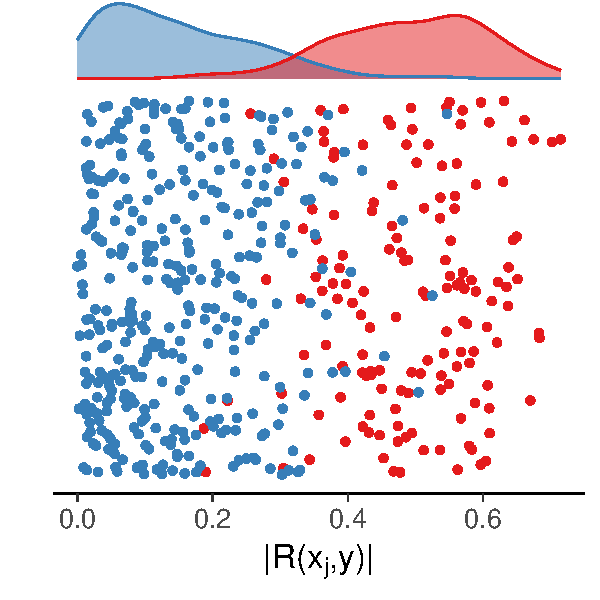
\includegraphics[width=5.5cm]{toy_corr1.pdf}\\
%   \vspace{-0.2cm}
%   \hspace{0.5cm} {\color{set12} irrelevant $x_j$}, {\color{set11} relevant $x_j$}\\
%   \vspace{0.2cm}
%   \hspace{0.5cm} Sample correlation with $y$\\
  
% \end{frame}

\begin{frame}{\only<1>{Knowing the latent values would help}\only<2>{Estimating the latent values with a reference}\uncover<2->{ model helps}}

  \hspace{-0.4cm}
  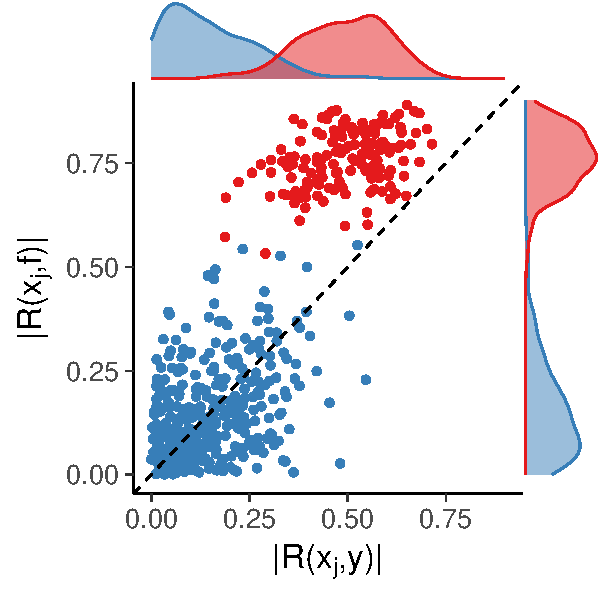
\includegraphics[width=5.5cm]{toy_corr2.pdf}
  \uncover<2->{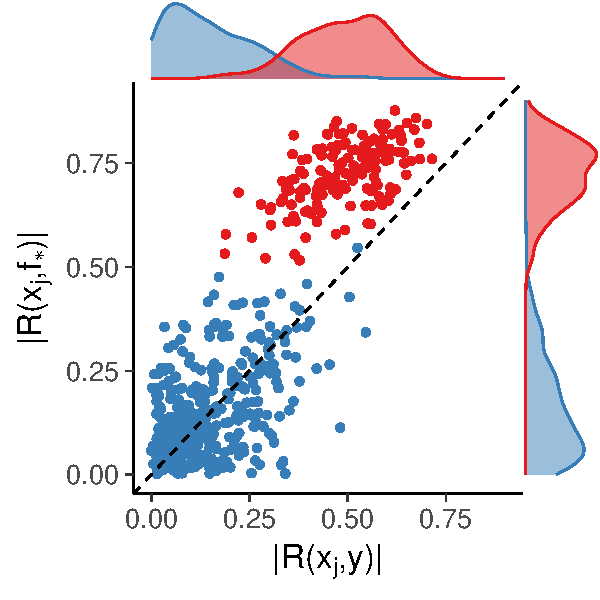
\includegraphics[width=5.5cm]{toy_corr3.pdf}}\\
  \vspace{-0.2cm}
  \hspace{0.5cm} {\color{set12} irrelevant $x_j$}, {\color{set11} relevant $x_j$}\\
  \vspace{0.2cm}
  A) Sample correlation with $y$ vs. sample correlation with $f$\\
  \uncover<2->{B) Sample correlation with $y$ vs. sample correlation with $f_*$\\
  % $f_* = $ linear regression fit with 3 supervised principal components}
  $f_* = $ linear regression fit with 3 principal components}
  
\end{frame}

\begin{frame}{Bayesian justification}
  
  \begin{itemize}
  \item  Theory says to integrate over all the uncertainties
    \begin{itemize}
    \item build a rich model
    \item make model checking etc.
    \item this model can be the reference model
    \end{itemize}
  \item<2-> Consider model selection as decision problem
  \item<3-> Replace full posterior {\color{set11} $p(\theta \mid D)$} with
    some constrained {\color{set12} $q(\theta)$} so that the {\color{set13} \emph{predictive
      distribution}} changes as little as possible
  \item<4-> Example constraints
    \begin{itemize}
    \item {\color{set12} $q(\theta)$} can have only point mass at some $\theta_0$ \\
      $\Rightarrow$ ``Optimal point estimates''
    \item<5-> Some covariates must have exactly zero regression coefficient \\
      $\Rightarrow$ ``Which covariates can be discarded''
    \item<6-> Much simpler model \\
      $\Rightarrow$ ``Easier explanation''
    \end{itemize}
\end{itemize}

\end{frame}

\begin{frame}{Logistic regression with two covariates}

  \vspace{\baselineskip}
  
  \begin{overlayarea}{\textwidth}{0.7\textwidth}
    \begin{minipage}{0.99\textwidth}
      \begin{center}
        \only<1>{ \minput{proj_posterior} }%
        \only<2>{ \minput{proj_b1b2_single} }%
        \only<3>{ \minput{proj_b2_single} }%
        \only<4>{ \minput{proj_b1_single} }%
        \only<5>{ \minput{proj_b2_dbd} }%
        \only<6>{ \minput{proj_b1_dbd} }%
      \end{center}
    \end{minipage}
    \begin{minipage}{0.99\textwidth}
      \only<1>{Full posterior for $\beta_1$ and $\beta_2$ and contours of predicted class probability}
      \only<2>{Projected point estimates for $\beta_1$ and $\beta_2$}
      \only<3>{Projected point estimates, constraint $\beta_1 = 0$}
      \only<4>{Projected point estimates, constraint $\beta_2 = 0$}
      \only<5>{Draw-by-draw projection, constraint $\beta_1 = 0$}
      \only<6>{Draw-by-draw projection, constraint $\beta_2 = 0$}
    \end{minipage}
  \end{overlayarea}
\end{frame}


\begin{frame}{Predictive projection}


  \begin{itemize}
  \item Replace full posterior {\color{set11} $p(\theta \mid D)$} with
    some constrained {\color{set12} $q(\theta)$} so that the {\color{set13} \emph{predictive
      distribution}} changes as little as possible
  \item<2-> As the full posterior {\color{set11} $p(\theta \mid D)$} is projected to {\color{set12} $q(\theta)$}
    \begin{itemize}
    \item the prior is also projected and there is no need to define
      priors for submodels separately
    \item<3-> even if we constrain some coefficients to be $0$, the
      predictive inference is conditoned on the information related
      features contributed to the reference model
    \item<4-> solves the problem of how to do the inference after the
      model selection
    \end{itemize}
  \end{itemize}

  
\end{frame}

\frame{

  {\Large\color{navyblue} Projective selection}

\begin{itemize}
	\item How to select a feature combination? \pause
	\item For a given model size, choose feature combination with minimal projective loss \pause
	\item Search heuristics, e.g. 
	\begin{itemize}
        \item Monte Carlo search
        \item Forward search
        \item $L_1$-penalization (as in Lasso)
	\end{itemize} \pause 
      \item Use cross-validation to select the appropriate model size
        \begin{itemize}
        \item need to cross-validate over the search paths
        \end{itemize}
      \end{itemize} 
}


\frame{

  {\Large\color{navyblue} Projective selection vs. Lasso}

Same simulated regression data as before, \\
$n=50$, $p=500$, $p_\text{rel} = 150$, $\rho=0.5$

\vspace{0.5em}

  \makebox[12.1cm][t]{
    \hspace{-0.5cm}
  \begin{minipage}{0.99\textwidth}
      \only<1>{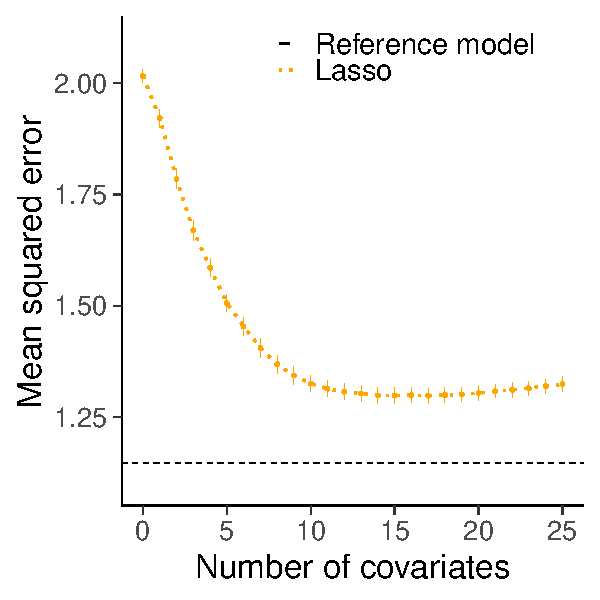
\includegraphics[width=5.5cm]{vslasso1rmse.pdf}}
      \only<2>{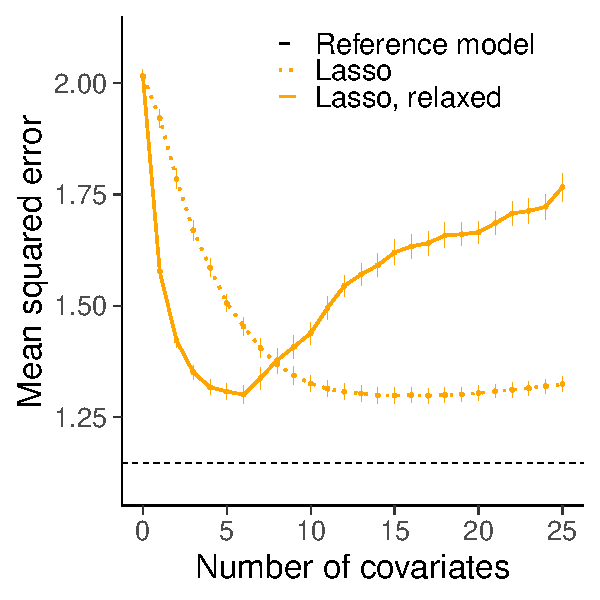
\includegraphics[width=5.5cm]{vslasso2rmse.pdf}}
      \only<3->{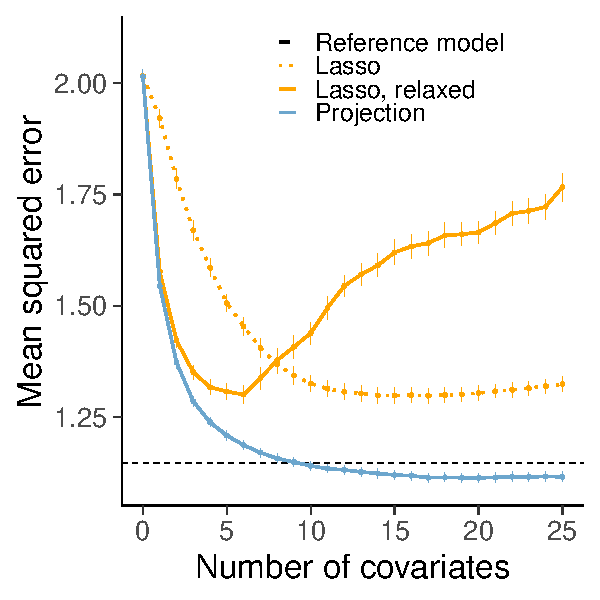
\includegraphics[width=5.5cm]{vslasso3rmse.pdf}}
      \uncover<4>{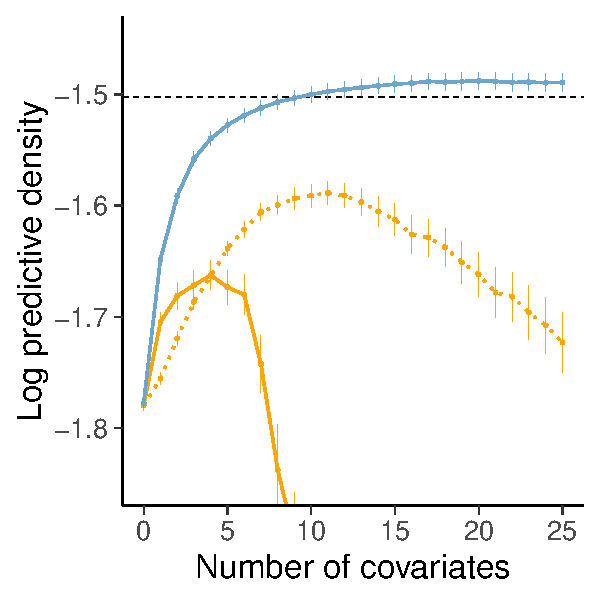
\includegraphics[width=5.5cm]{vslasso3mlpd.pdf}}
  \end{minipage}
  }
  
}

% \frame{

%   {\Large\color{navyblue} Real data benchmarks}\\
%   $n = 54...102$, $p=1536...22283$, Bayes SPC as the reference
% \begin{overlayarea}{\textwidth}{0.7\textwidth}
% \vspace{-0.5em}
% 	\begin{minipage}{0.99\textwidth}
% 	\begin{center}
%           \minput[pdf]{realdata}
% 	\end{center}
% 	% hidings
% 	\only<1>{ \hide[white]{-0.5}{-0.02}{0.42}{1.05} }%
% 	\only<2>{ \hide[white]{-0.3}{-0.02}{0.22}{1.05} }%
% 	\only<3>{ \hide[white]{-0.07}{-0.02}{0.01}{1.05} }%
	
% 	\end{minipage}
% 	%\begin{minipage}{0.99\textwidth}
% 	%\end{minipage}
	
% \end{overlayarea}
% }

% \frame{

%   {\Large\color{navyblue} Computation time}

%   \begin{table}%
%     \small
% \vspace{-0.2cm}
% \centering
% \abovetopsep=2pt
% \begin{tabular}{ lccrrrr }
% \toprule
% Data set & $n$ & $p$ & \multicolumn{4}{c}{Computation time} \\
% \cmidrule(r){4-7}
%  & & & Bayes SPC & Projection & Lasso1 & Lasso2 \\ 
% \midrule
% Ovarian & 54 & 1536 & 30.4 & 3.6 & 1.3 & 0.2  \\
% Colon & 62 & 2000 & 31.0 & 4.0 & 1.6 & 0.3  \\
% Prostate & 102 & 5966 & 49.4 & 7.6 & 5.0 & 0.8\\
% Leukemia & 72 & 7129 & 47.0 & 6.3 & 5.6 & 0.7  \\
% Glioma & 85 & 22283 & 95.8 & 14.2 & 15.6 & 2.6 \\
% \bottomrule
% \end{tabular}
% \caption{{\it Computation times:} Average computation time (in seconds) over five repeated runs. In all cases the time contains the cross-validation of the tuning parameters and/or the model size. The first result for Lasso is computed using our software ({\tt projpred}) whereas the second result (and that of ridge) is computed using the R-package {\tt glmnet} which is more highly optimized. }
% \label{tab:computation_times}
% \end{table}
% }

% \begin{frame}
  
%   {\Large\color{navyblue} More results}\\

%   {\footnotesize
%   \begin{itemize}
%   \item More results projpred vs. Lasso and elastic net:\\
%     Piironen, Paasiniemi, Vehtari (2018). Projective Inference in
%     High-dimensional Problems: Prediction and Feature Selection.
%     \href{https://arxiv.org/abs/arXiv:1810.02406}{arXiv:1810.02406}
%   \item<2-> More results projpred vs. marginal posterior probabilities:\\
%     Piironen and Vehtari (2017). Comparison of Bayesian predictive
%     methods for model selection. Statistics and Computing,
%     27(3):711-735.
%     \href{https://dx.doi.org/10.1007/s11222-016-9649-y}{doi:10.1007/s11222-016-9649-y}.
%   \item<3-> projpred for Gaussian graphical models:\\
%     Williams, Piironen, Vehtari, Rast (2018). Bayesian estimation of Gaussian graphical models with projection predictive selection. \href{https://arxiv.org/abs/1801.05725}{arXiv:1801.05725}
%   \item<4-> More results for Bayes SPC:\\
%     Piironen and Vehtari (2018). Iterative supervised principal components. 21st AISTATS, PMLR 84:106-114. \href{http://proceedings.mlr.press/v84/piironen18a.html}{Online}.
%   \item<5-> Several case studies for small to moderate dimensional ($p=4 \ldots 100$) small data:\\
%     Vehtari (2018). Model assesment, selection and inference after
%     selection. \url{https://avehtari.github.io/modelselection/}
%   \end{itemize}
%   }
% \end{frame}

\begin{frame}{Bodyfat: small $p$ example of projection predictive}
  
  Predict bodyfat percentage. The reference value is obtained by
  immersing person in water. $n=251$.

  \pause
  \vspace{-0.7\baselineskip}
  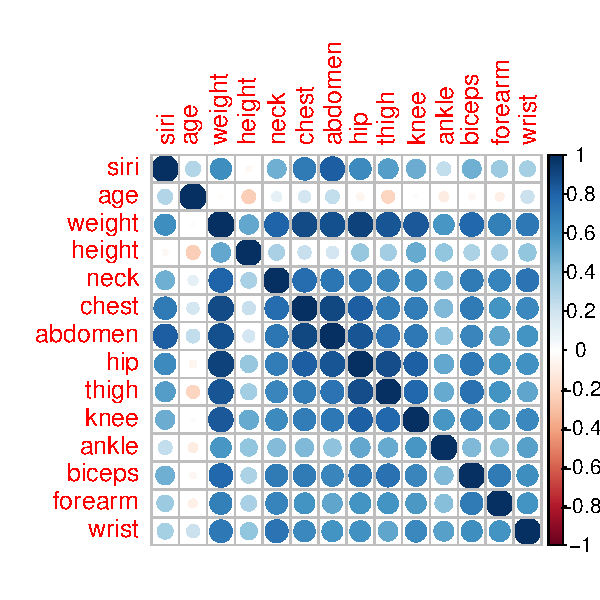
\includegraphics[width=7.7cm]{bodyfat_corr.pdf}

\end{frame}

\begin{frame}{Bodyfat}

  Marginal posteriors of coefficients
  
  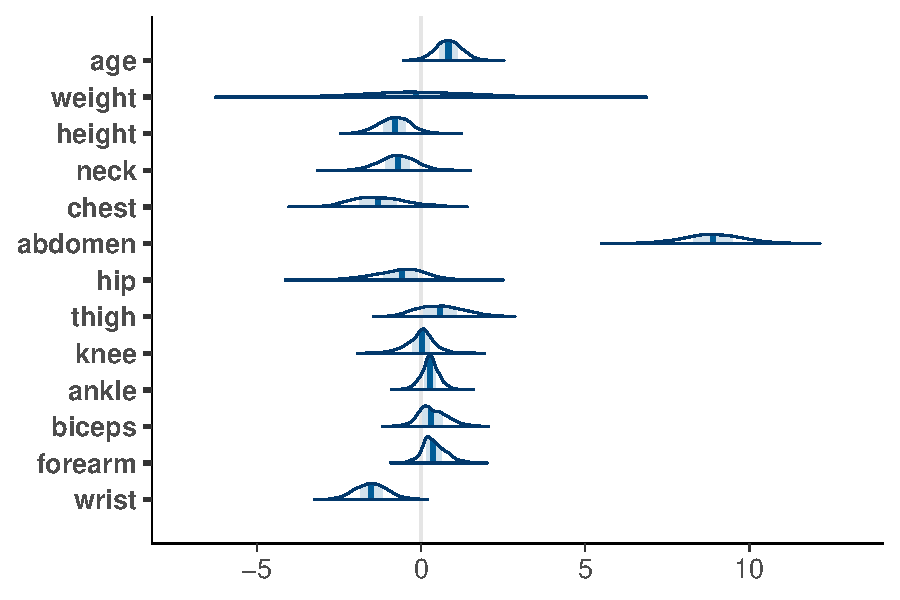
\includegraphics[width=11cm]{bodyfat_mcmc_areas.pdf}

\end{frame}

\begin{frame}{Bodyfat}

  Bivariate marginal of weight and height
  
  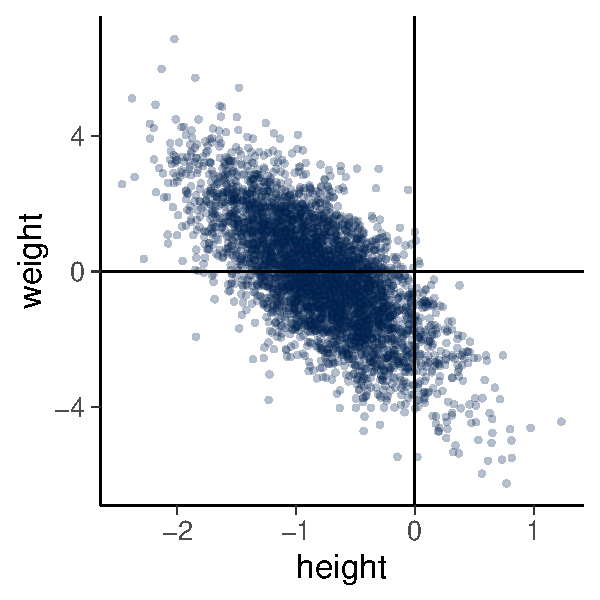
\includegraphics[width=7.5cm]{bodyfat_mcmc_scatter.pdf}

\end{frame}

\begin{frame}{Bodyfat}

  The predictive performance of the full and submodels
  
  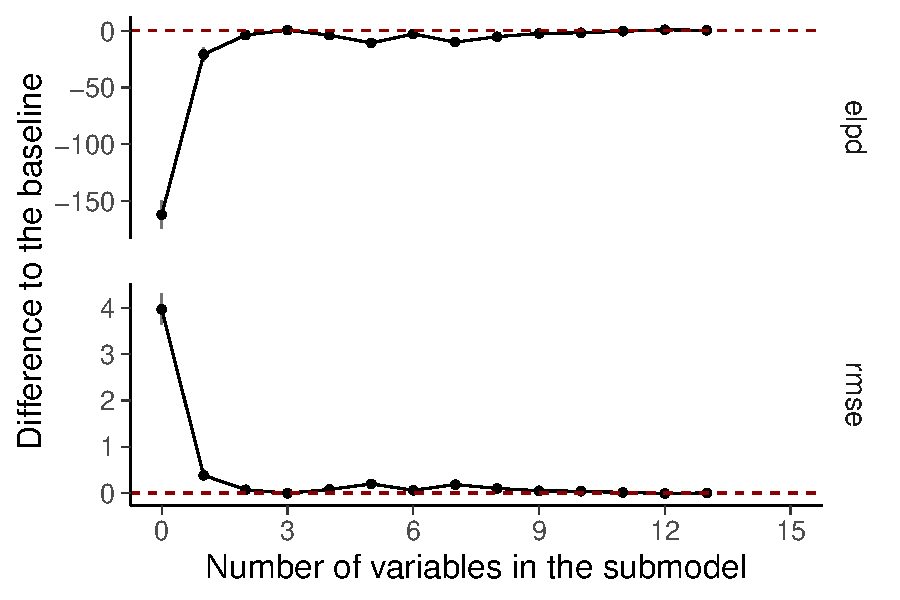
\includegraphics[width=11cm]{bodyfat_varsel_plot.pdf}

\end{frame}

\begin{frame}{Bodyfat}

  Marginals of the reference and projected posterior

  % TODO: side by side comaprison to original marginals
  \vspace{\baselineskip}
  
  \begin{minipage}[t]{1\linewidth}
    \hspace{-1cm}
    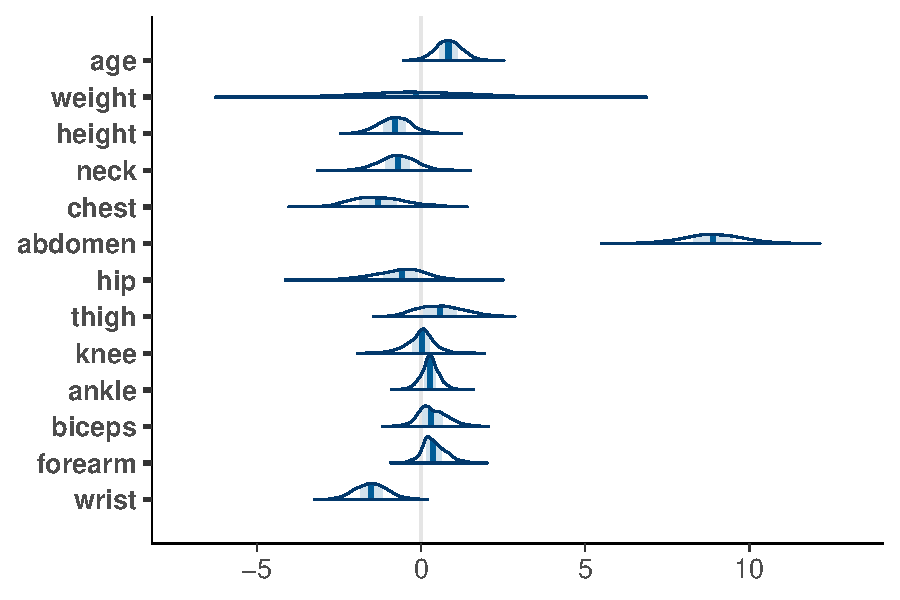
\includegraphics[width=6.5cm]{bodyfat_mcmc_areas.pdf}
  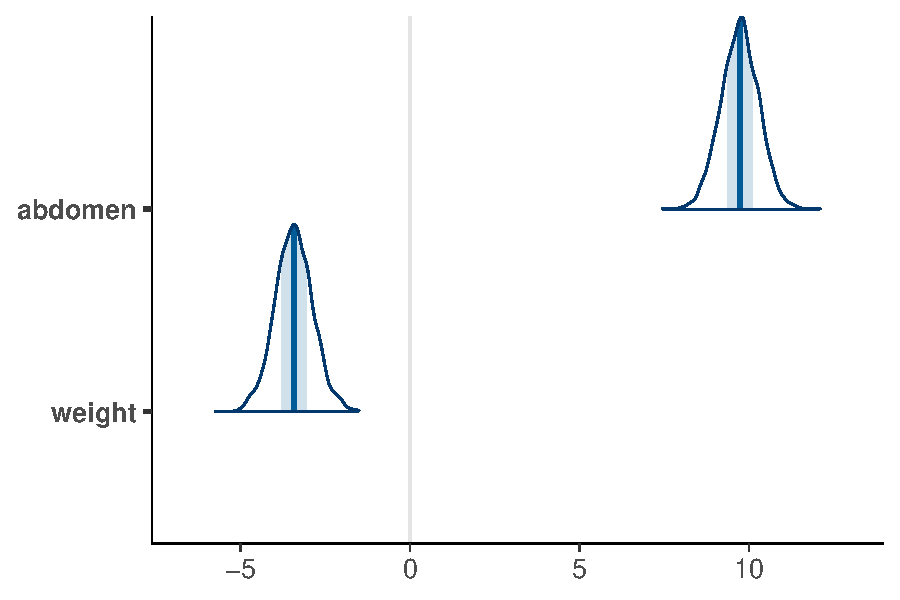
\includegraphics[width=6.5cm]{bodyfat_proj_mcmc_areas.pdf}
\end{minipage}
\end{frame}

\begin{frame}{Predictive performance vs. selected variables}

  \begin{itemize}
  \item<+-> The initial aim: find the minimal set of variables
    providing similar predictive performance as the reference model
  \item<+-> Some keep asking can it find the true variables
    \begin{itemize}
    \item<3-> What do you mean by true variables?
    \end{itemize}
  \end{itemize}

  \uncover<3>{
      \vspace{-0.5\baselineskip}
    \begin{minipage}[t]{1\linewidth}
      \hspace{-1cm}
  \vspace{-.88\baselineskip}
  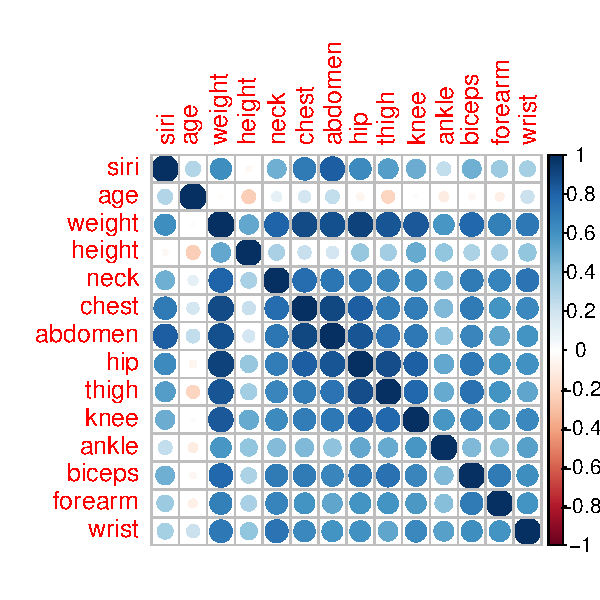
\includegraphics[width=6cm]{bodyfat_corr.pdf}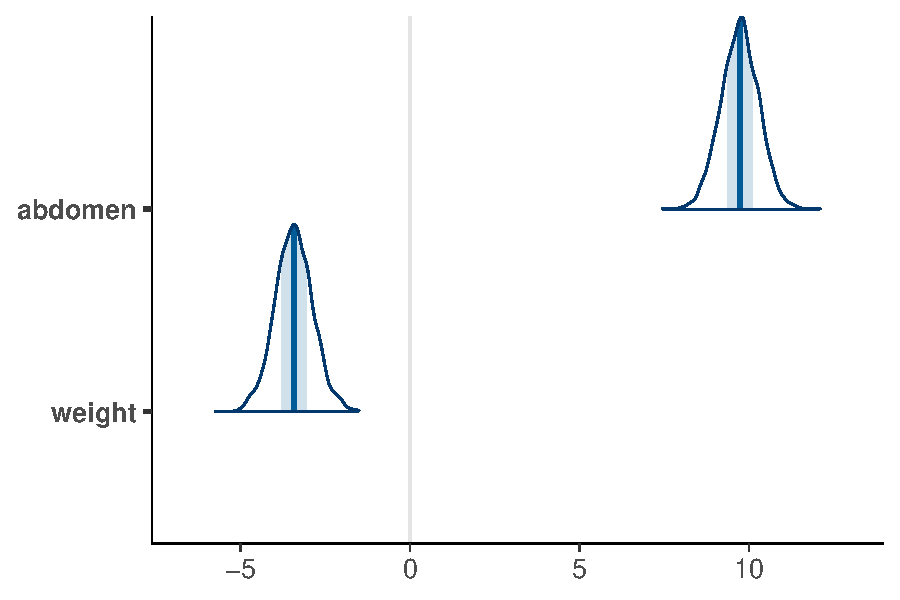
\includegraphics[width=6.5cm]{bodyfat_proj_mcmc_areas.pdf}
    \end{minipage}
}

\end{frame}

% \begin{frame}{Example: Individual correlations}

% \vspace{-1.5\baselineskip}
  
% \begin{minipage}[t]{0.3\linewidth}
% \begin{equation*}
% \begin{alignedat}{1}
%   f &  \sim \N(0,1),  \\
%   y \mid f &\sim \N(f, 1) 
% \end{alignedat}
% \end{equation*}
% \end{minipage}
%   \begin{minipage}[t]{0.4\linewidth}
% \begin{equation*}
% \begin{alignedat}{2}
%   x_j \mid f &\sim \N(\sqrt{\rho}f,\, 1-\rho), \qquad && j = 1,\dots,150 \,, \\
%   x_j \mid f &\sim \N(0, 1), && j = 151,\dots, 500 \,.
% \end{alignedat}
% \end{equation*}
% \end{minipage}
% \vspace{-0.2\baselineskip}

% \center
% {Correlation for $x_j,f_*$ ($f_*$ = PCA + linear regression)\\}
% \vspace{-0.5\baselineskip}
% \only<1>{\includegraphics[width=8cm]{Rfs.pdf}}\only<2>{\includegraphics[width=8cm]{Rfs1.pdf}}\only<3>{\includegraphics[width=8cm]{Rfs2.pdf}}

% \end{frame}

\begin{frame}{Variability under data perturbation}

   Comparing projection predictive variable selection (projpred)
    and stepwise maximum likelihood over bootstrapped datasets

  \vspace{-0.5\baselineskip}
  \begin{minipage}[t]{1\linewidth}
      \hspace{-1cm}
      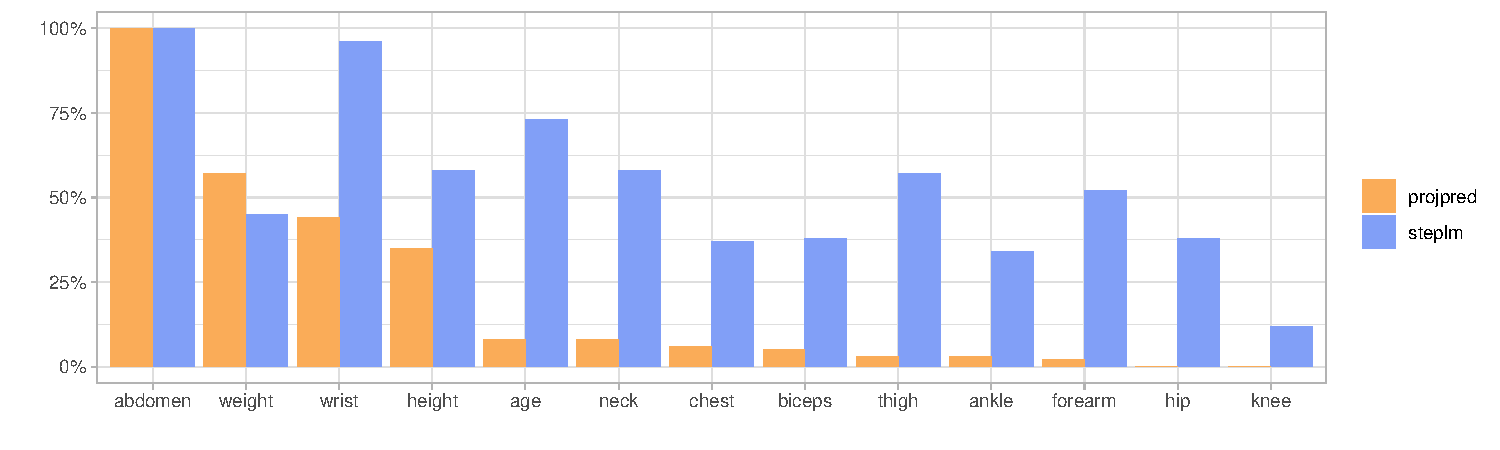
\includegraphics[width=12.5cm]{inc_prob.pdf}
    \end{minipage}
    \pause
  \begin{minipage}[t]{1\linewidth}
      \hspace{-0.9cm}
      \includegraphics[width=12.5cm]{bodyfat_table.png}
    \end{minipage}

  \end{frame}

  \begin{frame}{Variability under data perturbation}

   Comparing projection predictive variable selection (projpred)
    and stepwise maximum likelihood over bootstrapped datasets

  
  \vspace{-0.5\baselineskip}
  \begin{minipage}[t]{1\linewidth}
      \hspace{-1cm}
      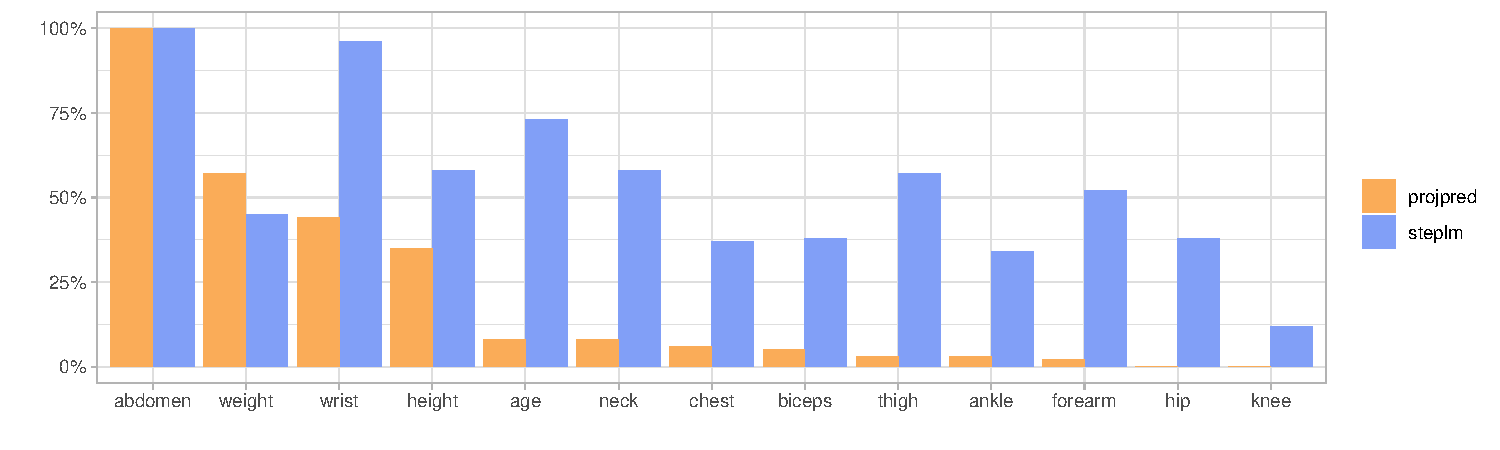
\includegraphics[width=12.5cm]{inc_prob.pdf}
    \end{minipage}
  
    \begin{itemize}
      \vspace{-1\baselineskip}
    \item<1-> Reduced variability, but in case of noisy finite data,
      there will be some variability under data perturbation
    \item<2-> projpred uses
      \begin{itemize}
      \item Bayesian inference for the reference
      \item \only<2>{The reference model}\only<3->{{\color{set13}The reference model}}
      \item Projection for submodel inference
      \end{itemize}
    \end{itemize}

  \end{frame}

% \begin{frame}{Predictive performance vs. selected variables}

%   \begin{itemize}
%   \item projpred has very good predictive performance and small false
%     discovery rate {\color{gray}(with simulated data with known truth)}
%   \item Other variable selection methods (e.g. steplm) can be improved
%     just by replacing the data with the predictions from the reference
%     model
%   \end{itemize}

%   \pause
% \vspace{1\baselineskip}
  
%   \begin{minipage}[t]{1\linewidth}
%       \hspace{-.9cm}
% \includegraphics[width=12.5cm]{rmse_vs_fdr_parallel.pdf}
% \end{minipage}  

% \end{frame}

% \begin{frame}{Complete variable selection}

%   \begin{itemize}
%   \item projpred can be used iteratively to search for all variables
%     with some predictive relevance
%   \item More challenging problem, where specialized algorithms seem to
%     perform better
%     \begin{itemize}
%     \item reference model helps to improve other methods, too
%     \end{itemize}
%   \end{itemize}
  
% \end{frame}

% \begin{frame}{Networks as a bunch of linear models}
  
%   \begin{center}
%     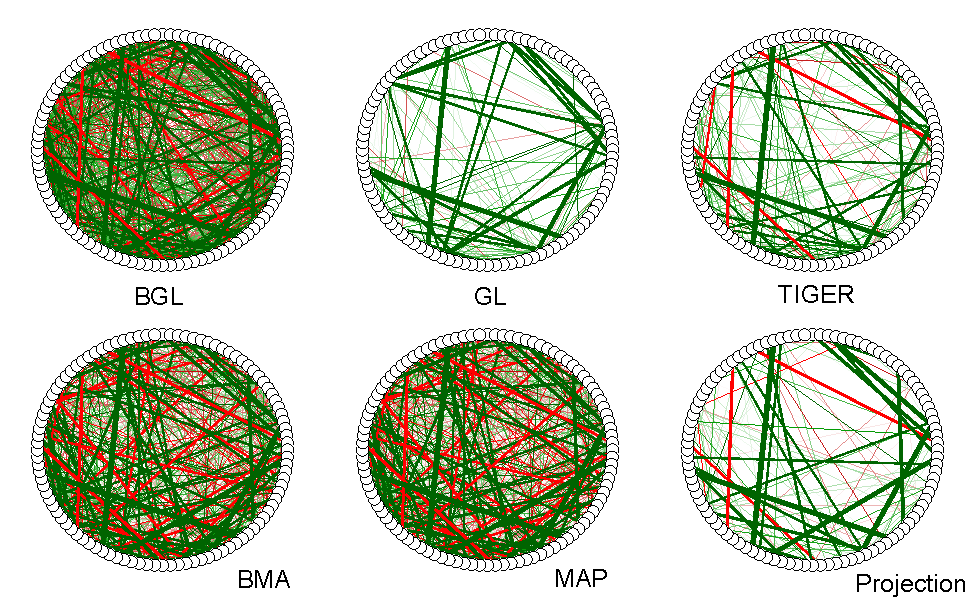
\includegraphics[width=8.5cm]{ceu.pdf}
%   \end{center}
%     {\footnotesize CEU genetic network. BGL: Bayesian glasso; GL: glasso;
%       TIGER: tuning insensitive graph estimation and regression; BMA:
%       Bayesian model averaging; MAP: Maximum a posteriori; Projection:
%       projection predictive selection.}

%       % \item Williams, Piironen, Vehtari, Rast (2018). Bayesian estimation of Gaussian graphical models with projection predictive selection. \href{https://arxiv.org/abs/1801.05725}{arXiv:1801.05725}\\

% \end{frame}

\begin{frame}{Multilevel regerssion and GAMMs}
  

  \begin{itemize}
  \item \texttt{projpred} supports also hierarchical models in \texttt{brms}\\
  {\small  Catalina, Bürkner, and Vehtari (2022). Projection predictive inference for generalized linear and additive multilevel models. \textit{Proceedings of the 24th International Conference on Artificial Intelligence and Statistics (AISTATS), PMLR} 151:4446–4461. \url{https://proceedings.mlr.press/v151/catalina22a.html}}
  \end{itemize}
  
\end{frame}

\begin{frame}{Scaling}

  \begin{itemize}
  \item So far the biggest number of variables we've tested is 22K
    \begin{itemize}
    \item 96s for creating a reference model
    \item 14s for projection predictive variable selection
    \end{itemize}
  \end{itemize}
  
\end{frame}

% \begin{frame}{In machine learning (example)}

%   \vspace{-0.3\baselineskip}
%   \begin{itemize}
%   \item BART integrates over the uncertainty producing many trees
%   \item CART makes just one tree which is easier to analyse
%   \item Projecting BART to CART gets benefits of both
%   \end{itemize}

%   \pause
%   \center
%   \vspace{-0.8\baselineskip}
%   \includegraphics[width=7.5cm]{CART_BART.png}

% \end{frame}

% \begin{frame}{Take-home messages}

% \begin{itemize}
% \item Good reference model filters out noise, making it easier to
%   search for simpler models
%   \begin{itemize}
%   \item Applicable for many algorithms and models
%   \end{itemize}
% \item Reference model + projection improve model selection
%   \begin{itemize}
%   \item Bayesian decision theoretical justification
%   \item Excellent tradeoff between accuracy and model complexity
%   \item Excellent FDR in minimal set selection
%   \item Can be useful also for identifying all the relevant features
%   \end{itemize}
% \end{itemize}

% \end{frame}

\begin{frame}[fragile]{Intro paper and brms and rstanarm + projpred examples}

\begin{itemize}
\item {\small McLatchie, Rögnvaldsson, Weber, and Aki Vehtari (2024). Advances in projection predictive inference. \emph{Statistical Science}. \url{https://arxiv.org/abs/2306.15581}}
\item \url{https://mc-stan.org/projpred/articles/projpred.html}
\item \url{https://users.aalto.fi/~ave/casestudies.html}
\item Fast and often sufficient if $n\gg p$\\
\begin{minted}[fontsize=\footnotesize]{r}
varsel <- cv_varsel(fit, method='forward', cv_method='loo',
                    validate_search=FALSE)
\end{minted}
\item Slower but needed if not $n\gg p$\\
\begin{minted}[fontsize=\footnotesize]{r}
varsel <- cv_varsel(fit, method='forward', cv_method='kfold', K=10,
                    validate_search=TRUE)
\end{minted}
\item If $p$ is very big\\
\begin{minted}[fontsize=\footnotesize]{r}
varsel <- cv_varsel(fit, method='L1', cv_method='kfold', K=5,
                    validate_search=TRUE)
\end{minted}
\end{itemize}

\end{frame}

% \begin{frame}{References}
% \vspace{-0.5\baselineskip}
  
%   \scriptsize
  
% \begin{itemize}
% \item[-] Piironen, Paasiniemi, and Vehtari (2020). Projective inference in high-dimensional problems: prediction and feature selection. \textit{Electronic Journal of Statistics}, 14(1):2155-2197. \url{https://doi.org/10.1214/20-EJS1711}
% \item[-] Pavone, Piironen, Bürkner, and Vehtari (2020). Using reference models in variable selection. arXiv preprint arXiv:2004.13118. \url{https://arxiv.org/abs/2004.13118}
% \item[-] Piironen and Vehtari (2016). Projection predictive input variable selection for Gaussian process models. \textit{2016 IEEE 26th International Workshop on Machine Learning for Signal Processing (MLSP)}, doi:10.1109/MLSP.2016.7738829. \url{https://dx.doi.org/10.1109/MLSP.2016.7738829}
% \item[-] Piironen and Vehtari (2017). Comparison of Bayesian predictive methods for model selection. \textit{Statistics and Computing}, 27(3):711-735. doi:10.1007/s11222-016-9649-y. \url{https://link.springer.com/article/10.1007/s11222-016-9649-y}
% \item[-] Afrabandpey, Peltola, Piironen, Vehtari, and Kaski (2019). Making Bayesian predictive models interpretable: A decision theoretic approach. \textit{arXiv preprint arXiv:1910.09358} \url{https://arxiv.org/abs/1910.09358}
% \item[-] Williams, Piironen, Vehtari, and Rast (2018). Bayesian estimation of Gaussian graphical models with projection predictive selection. \textit{arXiv preprint arXiv:1801.05725}. \url{https://arxiv.org/abs/1801.05725}
% \item[-] Piironen, Paasiniemi, Catalina and Vehtari (2020). projpred:
%   Projection Predictive Feature
%   Selection. \url{https://mc-stan.org/projpred}
% \end{itemize}
% \end{frame}

\end{document}

%%% Local Variables: 
%%% mode: latex
%%% TeX-master: t
%%% TeX-command-extra-options: "-shell-escape"
%%% End:
